\documentclass[journal, letterpaper]{IEEEtran}
\usepackage{listings}
\usepackage{fancyvrb}
\usepackage{framed}
\usepackage[listings,skins]{tcolorbox}
\usepackage[skipbelow=\topskip,skipabove=\topskip]{mdframed}
\usepackage{pbox}
\usepackage{graphicx}
\usepackage{url}
\usepackage{hyperref}
\usepackage{caption}
\linespread{1}
\usepackage{float}

\mdfsetup{roundcorner=0}
% Congyang: Added the geometry module to add the margin of bottom
\usepackage[top=1in, bottom=1.2in, left=0.7in, right=0.7in]{geometry}
% Congyang: Added the indent first module (and delete "\\" of every paragraph) to make it indent every paragraph.
\usepackage{indentfirst}

\begin{document}
\title{Highway Tollgates Traffic Flow Prediction}
\author{Congyang Wang, Fangyu Lin, Meng Li \\ Department of Computer Science, Department of Data Science -- Worcester Polytechnic Institute, MA, 01609 \\ Email: \{cwang8, flin, mli6\}@wpi.edu}
% Congyang: Added our emails
\maketitle

% The Abstract
\begin{abstract} 
\large
As urban population and economy grow, automobile penetration in urban area, especially metropolises, has increased fast. As a result, traffic congestion problem has arisen not only within cities, but also in suburb such as areas bridging highways. The highway is therefore no longer highway due to congestion. In this paper, our goal is to predict the average travel time from one intersection to a tollgate, as well as predict traffic volume passing through tollgates in 20-minute windows, especially during the rush hours. We are going to use ARIMA models to do the prediction of volume and travel time with data collected in the previous time window. 

\end{abstract}

% The Keywords 
\begin{IEEEkeywords}
Traffic Prediction;
Traffic Flow Optimization;
Travel Time \& Traffic Volume Prediction
\end{IEEEkeywords}

\section{Introduction}
\large
%As the increase of population and economy, many people prefer to buy a house and live in another cities in Massachusetts. The price of apartments or houses in the cities are much more expensive than other small town, or cities. Definitely, the highway becomes the most important transportation way which connecting their homes to the working place. However, As the population increase, the number of vehicles cause the traffic congestion in the highway which makes uncomfortable to the drivers in daily life working schedule. For example, more people choose to take the Train from "Union Station" in Worcester to the "South Station" in Boston, which takes about 90 minutes (Comparing with normal average travel time 60 minutes).

Urbanization has been a global trend in recent decades, since it does not only benefit rural residents by improving accessibility of urban services and resources, the local economy also has gained momentum from the process. However, various problems have been engendered as concomitants. Inevitably, living costs surge as urban population grows and overcrowding worsens living conditions. As a consequence, a growing number of citizens choose to move to satellite towns and commute on highways. The shift in lifestyle choice intensifies pressures on highway management, since increase of traffic volume may cause congestions and lower highway performance. This, as a result, entails studies on highway traffic flows.

Highway tollgates are gateways implemented for toll collection so that highway construction costs and maintenance expenditures can be reimbursed, whereas they frequently act as blockades that cause traffic congestions, especially during rush hours and public holidays, and hence incur criticism towards the administration agency. To improve highway customer satisfaction and enhance highway performance, it is necessary to solve or at least mitigate the congestion problem caused by tollgates.  

Traffic volume prediction at tollgates enables administrators to make preparation in advance for digesting incoming high traffic volume, such as opening additional toll booths. Similarly, travel time prediction between tollgates and intersections empowers travelers to make choices over highway entrances, instead of running into dead-stop bumper-to-bumper situations unawarely. Moreover, with predicted traffic volume and travel time to a given tollgate, highway administration agency is able to regulate its upstream traffic flow to reduce chances of traffic congestion.

\section{Related Work}
\large
There is one similar research paper [3] which evaluates the electric auto-pay system and the manual pay system. As we all know that Massachusetts highway has implemented the electric auto-pay system since 1998, which is known as "E-ZPass". However, the tollgates were not removed until 2016. Then all tollgates have been removed in Massachusetts which improved the highway traffic average speed amazingly. In this paper, we assume that there is no manual tollgates at Tollgate one, two, and three for both the entry and exit direction. 

There are many good methodologies cited by other research papers. One [7] uses a loglinear model to predict the travel time in the highway. Another one [6] uses the Seasonal ARIMA Model to predict the highway volume producing more accurate results. One [4] considers the highway traffic as a multi-lane tollgates model. As we will consider the different effectiveness from the number of lanes in the tollgates, we have the data table three(links). The paper [4] considers the multi-lane as single lane to improve the average traffic velocity. Additionally, the paper [8] uses the Takagi–Sugeno–Kang Fuzzy Neural Network(TSKFNN) approach to predict the average travel time on highway and uses the back propagation neural network(BPNN) and the time series model (ARIMA) with the training trajectory data and validation trajectory data. 

\section{Methodology}
\large
\subsection{Problem Setting}
To study the efficiency of the highway traffic, we select a intersections and tollgates pairs as the target area. The Fig. \ref{fig:1} shows the detail of intersections and tollgates pairs graph. There are total six routes:

   a. Routes from Intersection A to Tollgates 2 \& 3;
   
   b. Routes from Intersection B to Tollgates 1 \& 3;
   
   c. Routes from Intersection C to Tollgates 1 \& 3.
   
\begin{figure} [H]
  \centering
  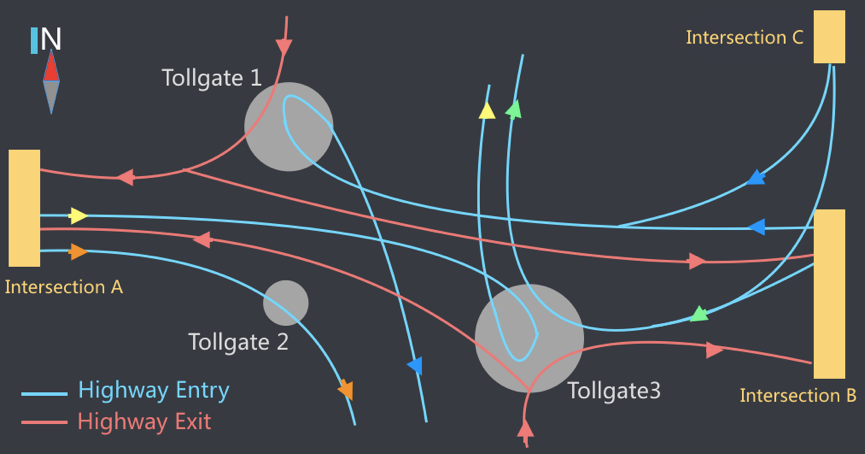
\includegraphics[width=0.48\textwidth]{road_graph.png}
  \caption{Intersection and Tollgate Network Graph}
  \label{fig:1}
\end{figure}

The road network in Fig. \ref{fig:1} here used the direction graph formed by road links with interconnected. Every route in this road network is represented by a sequence of links like the model you can see in Fig. 2.

So, We divide this problem into two tasks: 

	Task 1: To estimate the average travel time from designated intersections to tollgates. 
    
    Task 2: To predict average tollgate traffic volume.

In the task 1, we choose the 20-minutes time window, try to estimate the average travel time of vehicles for every specific route shown in Fig. 1 with our prediction models, so we will predict six average travel time for all routes. In the task 2, we focus on the tollgate volume prediction, we choose the 20-minutes time window as usual, try to predict the entry and exit tollgate volumes at tollgates 1,2 and 3 (tollgate 2 only has Highway Entry as shown in Fig. 1). Therefore, we will predict the volumes for the 5 tollgate-direction pairs in total.

\begin{figure} [t]
  \centering
  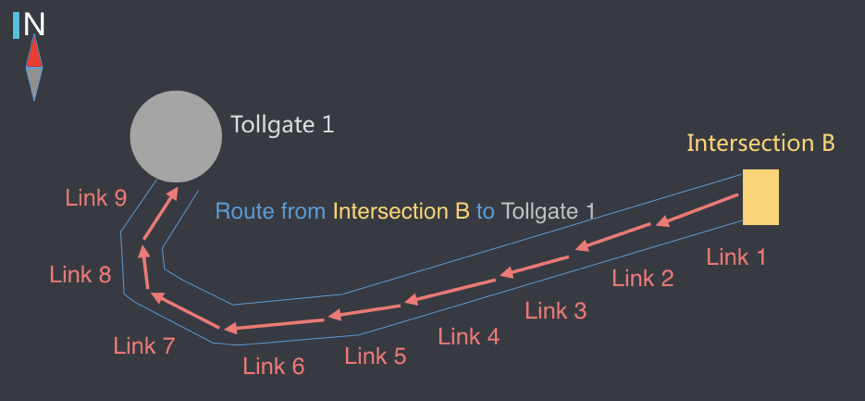
\includegraphics[width=0.48\textwidth]{link-sequence.png}
  \caption{Intersection and Tollgate Links Sequence}
  \label{fig:2}
\end{figure}

\begin{figure} [H]
  \centering
  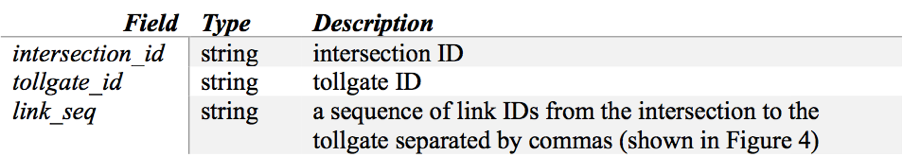
\includegraphics[width=0.48\textwidth]{route.png}
  \caption{Routes from Intersections to Tollgates}
  \label{fig:3}
\end{figure}

\subsection{Data Description}

There are five datasets we choose in training process. Two for time-invariable conditions and three for time-variable factors. 

The invariable data table (Fig. 3) includes the link sequence from intersections to tollgates, the graph like Fig. 2, the vehicles traveling from road intersections to highway tollgates have limited options, for each intersection-tollgate pair, this dataset selected the most important one. The data table (Fig. 4) which shows more details about infrastructure design of every piece of road link, the Fig. 5 also show the instruction of the links connection. 

For the time-variable factors like vehicle trajectories data (Fig. 6), traffic volume data (Fig. 7), weather data (Fig. 8). The trajectories data includes the time-stamped records of actual vehicles along the routes in Fig. 3. The traffic volume data with the records from the three tollgates. The weather data has the features which may effect the highway traffic with 3 hour time interval.



\begin{figure} [H]
  \centering
  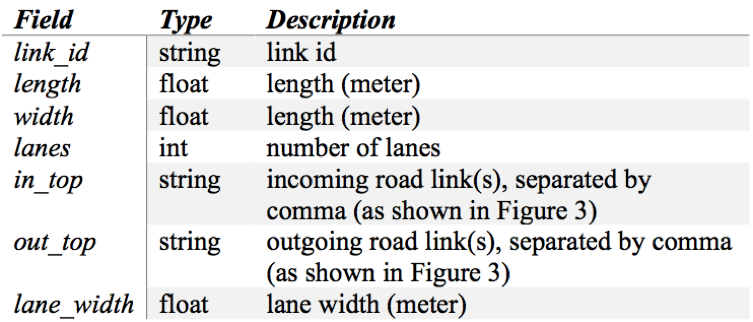
\includegraphics[width=0.48\textwidth]{road-link.png}
  \caption{Road Link Properties}
  \label{fig:4}
\end{figure}
\begin{figure} [H]
  \centering
  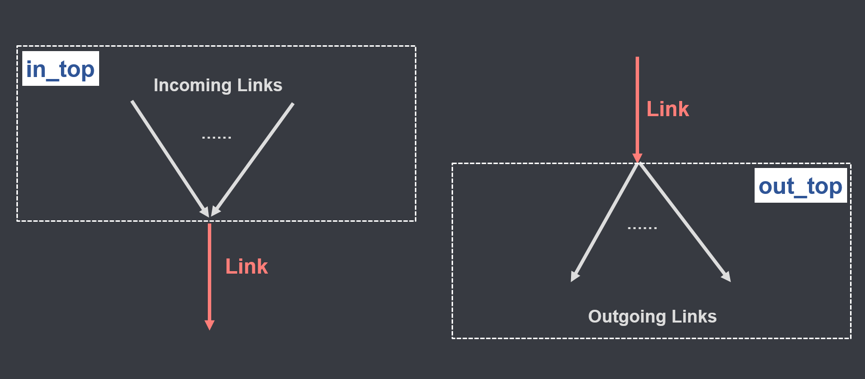
\includegraphics[width=0.48\textwidth]{in-out.png}
  \caption{Linkage In-top and Out-top Description}
  \label{fig:5}
\end{figure}

\begin{figure} [H]
  \centering
  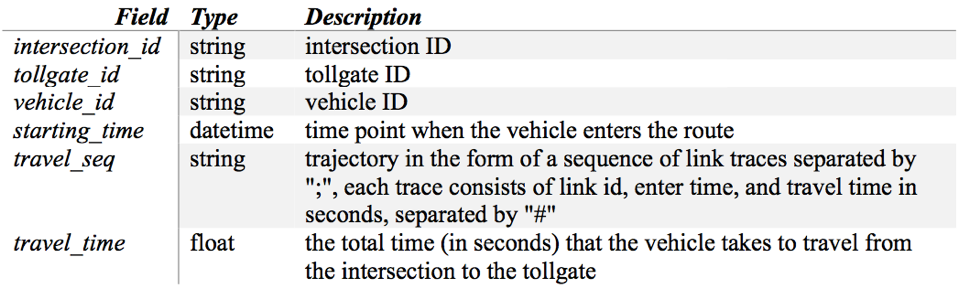
\includegraphics[width=0.48\textwidth]{trajectories.png}
  \caption{Vehicle Trajectories}
  \label{fig:6}
\end{figure}

\begin{figure} [H]
  \centering
  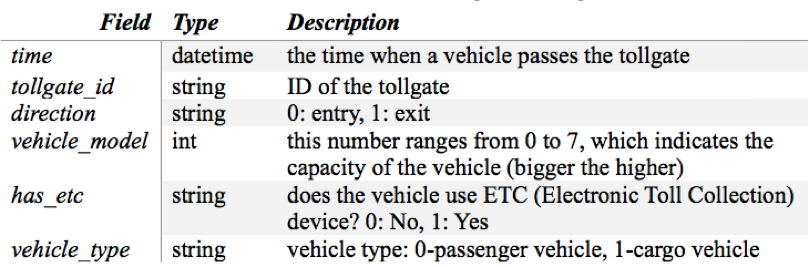
\includegraphics[width=0.48\textwidth]{volume.png}
  \caption{Traffic Volume through the Tollgates}
  \label{fig:7}
\end{figure}

\begin{figure} [H]
  \centering
  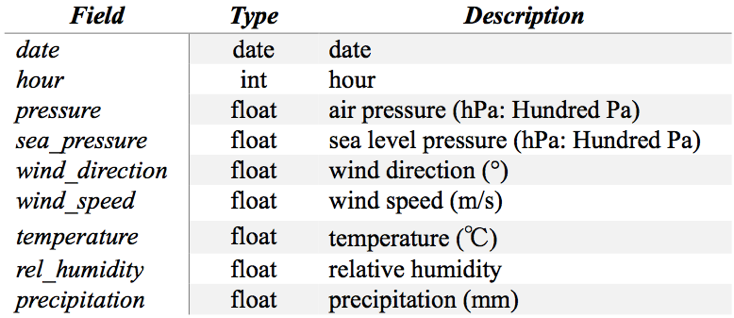
\includegraphics[width=0.48\textwidth]{weather.png}
  \caption{Weather in Target Area}
  \label{fig:8}
\end{figure}

\subsection{Preliminary Statistics}
To explore traffic volume pattern at each tollgate, the data are partitioned into uniform time slots of 20 minutes and visualized. 

\begin{figure} [H]
  \centering
  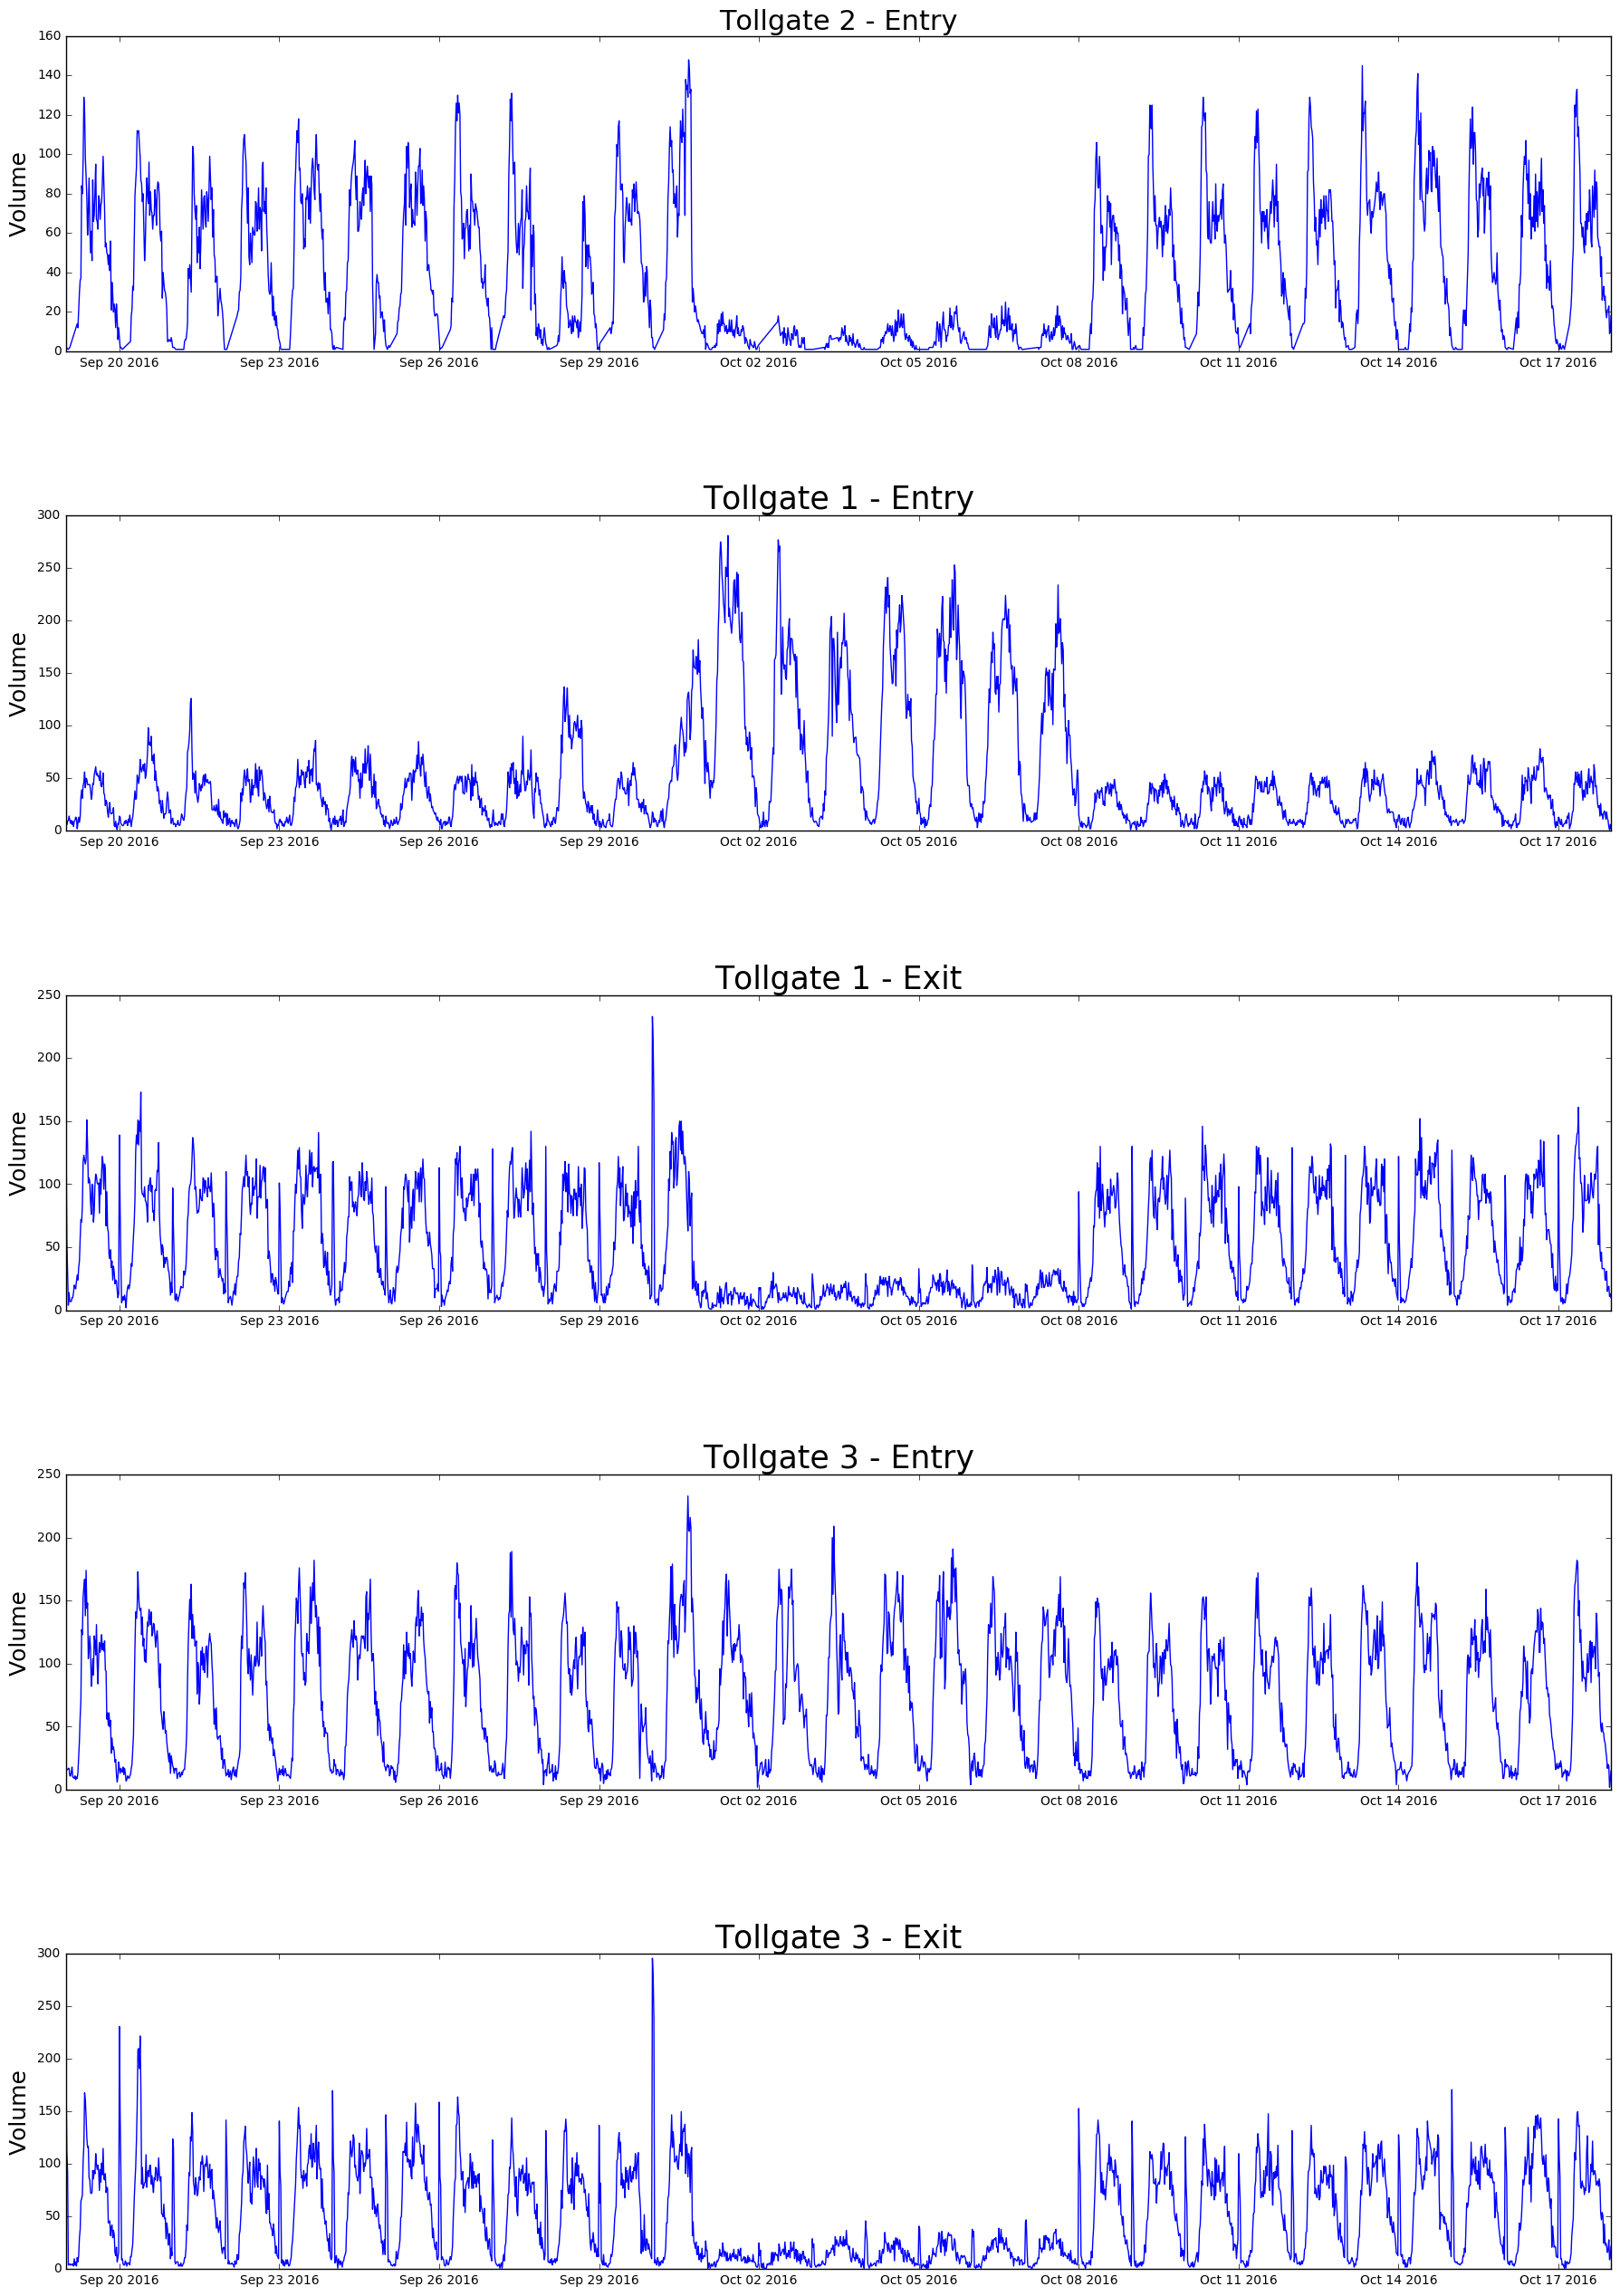
\includegraphics[width=0.35\textwidth]{tollgate-volume-3.png}
  \caption{Average Traffic Volume of Tollgate-Direction Pair Over Time}
  \captionsetup{justification=centering}
  \label{fig:9}
\end{figure} 

The Fig. \ref{fig:9} shows average traffic volumes in 20-minute windows versus time for each tollgate-direction pair. Apparently, average traffic volumes during October 1 to October 7 have very different patterns, compared to volumes in other time periods, except for the tollgate 3. In addition, two peaks per day are observed, in line with empirical observations that there are in general two rush-hour periods everyday.         

Fig. \ref{fig:10} shows average travel time in 20-minute windows from intersections to tollgates. The travel time is measured in seconds. For all intersection-tollgate pairs, the average travel time reveals a pattern that is approximately random. 

To figure out reasons why a large number of anomalies appear, we took a close look at some records with high travel time. We discovered that travel time of the last link of a route, i.e., the link to tollgates, dominated the overall travel time in some cases. 

\begin{figure} [H]
  \centering
  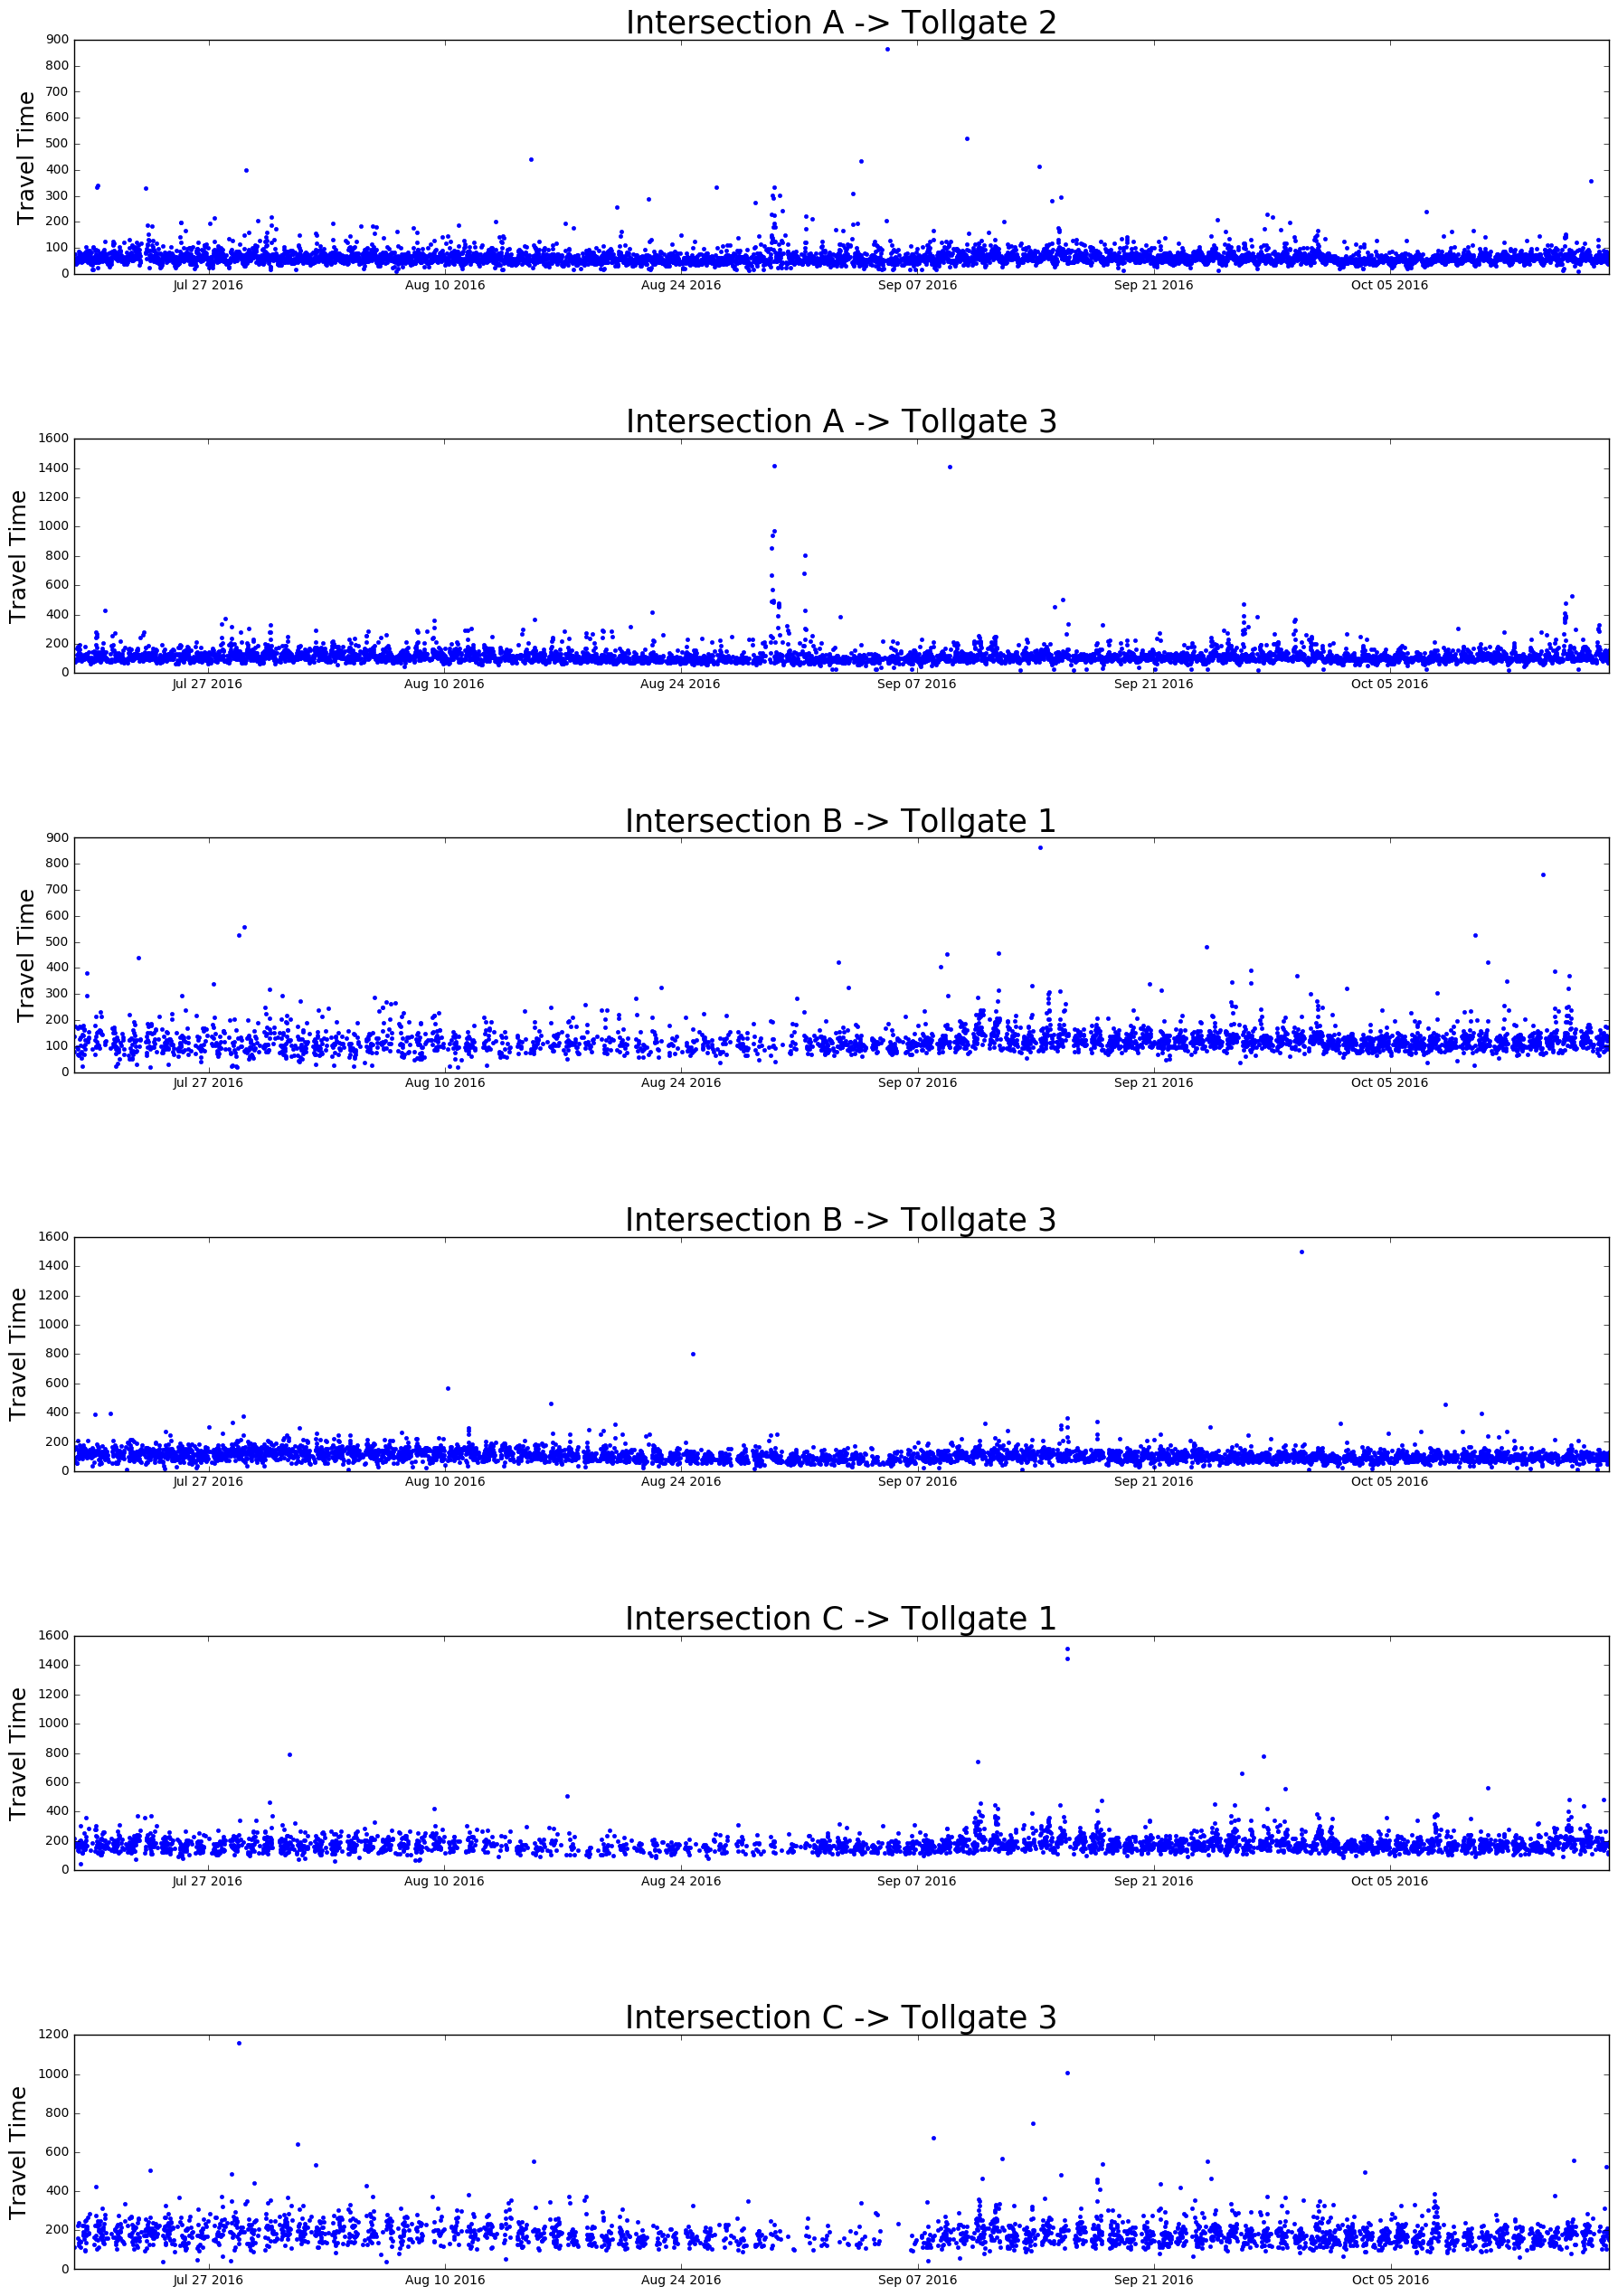
\includegraphics[width=0.35\textwidth]{intersection-tollgate-time-2.png}
  \caption{Average Travel Time from Intersections to Tollgates Over Time}
  \captionsetup{justification=centering}
  \label{fig:10}
\end{figure}

Then we came up with a hypothesis that the overall travel time was impacted by traffic volume at tollgates. Specifically, when traffic volume exceeds tollgate capacity, traffic congestion will arise and consequently, overall travel time from intersections to tollgates will increase because of queuing. However, in the case where traffic volume does not reach tollgate capacity, the overall travel time is not supposed to increase as traffic volume grows. 

To test the hypothesis, we plotted traffic volume versus travel time in the same time window at the same tollgate. The data records selected for the plot are those with the 10\% highest travel time from the intersection to the tollgate shown in plot titles, since tollgate capacities are unknown and it is unnecessary to put efforts into estimating them in the exploratory step. Any positive trend either linear or nonlinear will justify the hypothesis. However, Fig. \ref{fig:11} does not render any recognizable pattern, suggesting very weak relationship between traffic volume and travel time. To our surprise, high travel time appears even though traffic volume is extremely low. Therefore, the hypothesis is rejected and there must be other reasons that contribute to the anomalies and uncommon data pattern, which calls for further investigation. 

\begin{figure} [H]
  \centering
  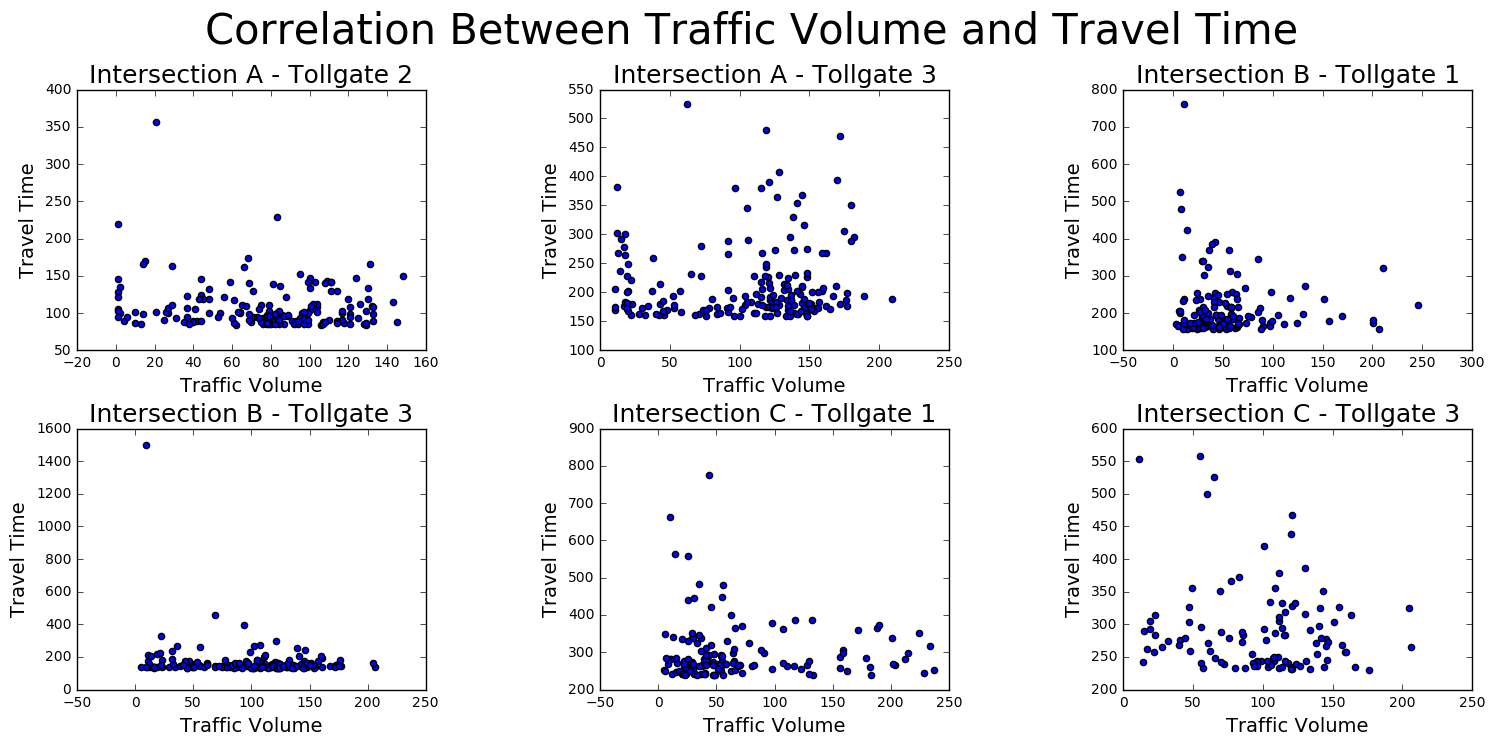
\includegraphics[width=0.48\textwidth]{corr_volume_time.png}
  \caption{Correlation Between Traffic Volume And Travel Time}
  \captionsetup{justification=centering}
  \label{fig:11}
\end{figure} 

\section{Experiments}
\large
%aa\\
\subsection{Time Window}

\begin{figure} [H]
  \centering
  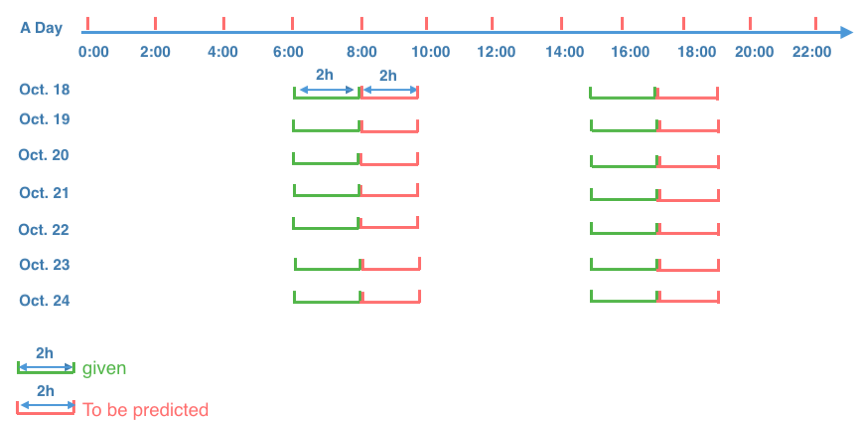
\includegraphics[width=0.48\textwidth]{time-window.png}
  \caption{Time Window}
  \label{fig:12}
\end{figure}

\subsection{Evaluation Metrics}

We choose Mean Absolute Percentage Error (MAPE) to evaluate the result. 
For task 1: We let $d_{rt}$ and $p_{rt}$ be the actual and predicted average travel time for route r during time window t. 

For task 2: We let C be the number of tollgate-direction pairs (as aforementioned: 1-entry, 1-exit, 2-entry, 3-entry and 3-exit), T be the number of time windows in the testing period, and $f_{ct}$ and $p_{ct}$ be the actual and predicted traffic volume for a specific tollgate-direction pair c during time window t. 

R and T are the number of routes and number of to-predict time windows in the testing period respectively.

The MAPE for travel time \& traffic volume prediction are defined as:

\begin{figure} [H]
  \centering
  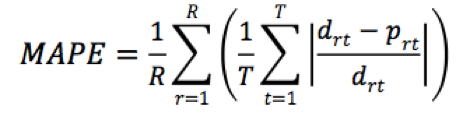
\includegraphics[width=0.2\textwidth]{MAPE.png}
  
  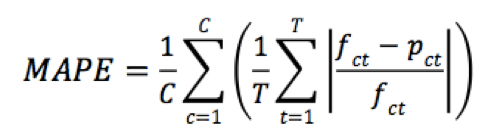
\includegraphics[width=0.2\textwidth]{MAPE-2.png}
  \caption{Evaluation Metrics}
  \captionsetup{justification=centering}
  \label{fig:13}
\end{figure}

\subsection{Result Analysis}

\section{Conclusions}
\large

\section{Schedule}
\large
\subsection{Milestone}
The table below shows the timeline for this project. We are going to follow our schedule to complete each milestone on time.
\begin{table}[ht]
%\caption{} % title of Table
\centering % used for centering table
\begin{tabular}{c| c| c} % centered columns (4 columns)
\hline\hline %inserts double horizontal lines
Date & Milestone & Description of Work  \\  % inserts table
%heading
\hline % inserts single horizontal line
Mar 15 & Proposal Complete & 2-3 Pages  \\ % inserting body of the table 
\hline
Mar 22 & Methodology For task-1 & Methodology Due  \\
\hline
Mar 29 & Training Result Due & Training Model  \\
\hline
April 05 & Evaluation Result Due & MAPE Result  \\  % [1ex] adds vertical space
\hline
April 12 & Training Result task-2 & Training Model \\
\hline
April 19 & Evaluation Result Due & MAPE Result \\
\hline
April 26 & Final Paper Presentation & Turn In \\
\hline %inserts single line
\end{tabular}
\label{table:nonlin} % is used to refer this table in the text
\end{table}

\subsection{Schedule}

\begin{figure} [H]
  \centering
  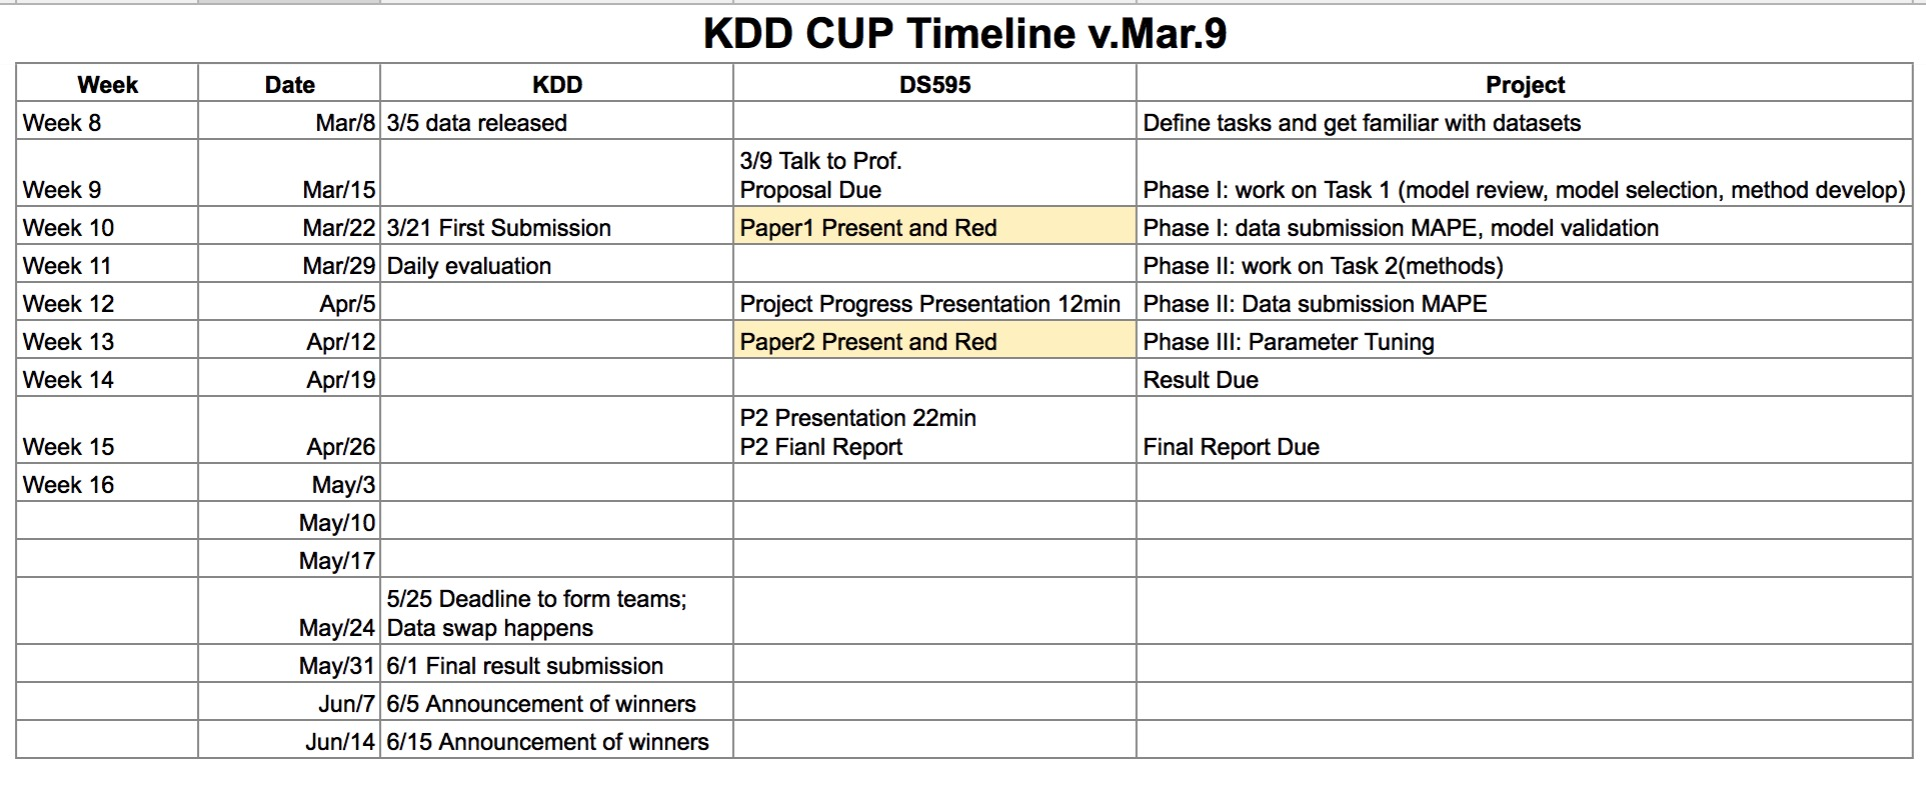
\includegraphics[width=0.49\textwidth]{KDDCUP-Schedule.jpg}
  \caption{Schedule}
  \label{fig:14}
\end{figure}

\begin{thebibliography}{99}
% \large 
\bibitem{c1}G. Wu, Y. Ding, Y. Li, J. Bao, Y. Zheng, and J. Luo, “Mining Spatio-Temporal Reachable Regions over Massive Trajectory Data,” pp. 1–12, Oct. 2016.
\bibitem{c2}Y. Ding, Y. Li, K. Deng, H. Tan, M. Yuan, and L. M. Ni, “Detecting and Analyzing Urban Regions with High Impact of Weather Change on Transport,” IEEE Transactions on Big Data, vol. PP, no. 99, pp. 1–1, 2016.
\bibitem{c3}Z. Liu-Hua, C. Shi-Dong, K. Ling-Jiang, and L. Mu-Ren, “The influence of tollbooths on highway traffic,” 2007.
\bibitem{c4}K. Komada and T. Nagatani, “Traffic flow through multi-lane tollbooths on a toll highway,” Physica A: Statistical Mechanics and its Applications, vol. 389, no. 11, pp. 2268–2279, Jun. 2010.
\bibitem{c5}Shi Fang, K. Bian, and K. Xie, “Vulnerability analysis of highway traffic networks using origin-destination tollgate data,” presented at the 2016 IEEE 19th International Conference on Intelligent Transportation Systems (ITSC), 2016, pp. 1957–1963.
\bibitem{c6}M. Tong and H. Xue, “Highway Traffic Volume Forecasting Based on Seasonal ARIMA Model,” Journal of Highway and Transportation Research and Development (English Edition), vol. 3, no. 2, pp. 109–112, Dec. 2008.
\bibitem{c7}L. Huang and M. Barth, “A Novel Loglinear Model for Freeway Travel Time Prediction,” presented at the 2008 11th International IEEE Conference on Intelligent Transportation Systems (ITSC), 2008, pp. 210–215.
\bibitem{c8}Y. Zhang and H. Ge, “Freeway Travel Time Prediction Using Takagi-Sugeno-Kang Fuzzy Neural Network,” Computer-Aided Civil and Infrastructure Engineering, vol. 28, no. 8, pp. 594–603, May 2013.
\bibitem{c9}W. Qiao, A. Haghani, C.-F. Shao, and J. Liu, “Freeway path travel time prediction based on heterogeneous traffic data through nonparametric model,” Journal of Intelligent Transportation Systems, vol. 20, no. 5, pp. 438–448, Sep. 2015.
\bibitem{c10}C.-S. Li and M.-C. Chen, “A data mining based approach for travel time prediction in freeway with non-recurrent congestion,” Neurocomputing, vol. 133, pp. 74–83, Jun. 2014.
\bibitem{c11}X. Xing, D. Yu, X. Tian, and Z. Cheng, “Freeway travel time prediction based on clustering method with data mining,” pp. 1–6, Sep. 2016.
\bibitem{c12}M. Tong and H. Xue, “Highway Traffic Volume Forecasting Based on Seasonal ARIMA Model,” Journal of Highway and Transportation Research and Development (English Edition), vol. 3, no. 2, pp. 109–112, Dec. 2008.
\bibitem{c13}J. Liu, L. Sun, W. Chen, and H. Xiong, “Rebalancing Bike Sharing Systems,” presented at the Proceedings of the 22nd ACM SIGKDD International Conference on Knowledge Discovery and Data Mining - KDD '16, 2016.


\end{thebibliography}

\end{document}